\documentclass[conference]{IEEEtran}
\IEEEoverridecommandlockouts

\usepackage{cite}
\usepackage{amsmath,amssymb,amsfonts}
\usepackage{algorithmic}
\usepackage{graphicx}
\usepackage{textcomp}
\usepackage{xcolor}
\usepackage{algorithm}
\usepackage[noend]{algpseudocode}
\usepackage{mathtools}
\usepackage{array}
\usepackage{multirow}
\usepackage{booktabs}
\usepackage{hyperref}
\usepackage{bm}
\usepackage{tabularx}
\usepackage{siunitx}
\usepackage{balance}
\usepackage{lipsum}
\usepackage{subcaption}
\usepackage{float}
\usepackage{tikz}
\usepackage{pgfplots}
\usepackage{listings}

\def\BibTeX{{\rm B\kern-.05em{\sc i\kern-.025em b}\kern-.08em
    T\kern-.1667em\lower.7ex\hbox{E}\kern-.125emX}}

\pgfplotsset{compat=1.18}
\usepgfplotslibrary{dateplot}

\begin{document}

\title{FALCON: Financial AnaLysis with Cross-asset Optimization Network for Portfolio Management}

\author{\IEEEauthorblockN{Chhatresh Sehgal}
\IEEEauthorblockA{\textit{Department of Computer Science} \\
\textit{University of Nottingham, Malaysia}\\
email: hfycs2@notttingham.edu.my}
\and
\IEEEauthorblockN{Youssef Mohamed Abdelhamid Mohamed}
\IEEEauthorblockA{\textit{Department of Computer Science} \\
\textit{University of Nottingham, Malaysia}\\
email: XXXXX@notttingham.edu.my}
}

\maketitle

\begin{abstract}
This paper introduces FALCON (Financial AnaLysis with Cross-asset Optimization Network), a novel deep learning architecture for multi-stock prediction and portfolio optimisation. FALCON leverages transformer networks with a hierarchical design incorporating asset-specific encoders, cross-asset attention mechanisms, and a portfolio optimisation agent. The system processes historical stock data to extract temporal patterns and cross-asset relationships, detect market regimes, and optimise portfolio allocations. Our framework combines individual asset analysis with cross-market context to provide robust investment strategies that adapt to changing market conditions. Experiments conducted on S\&P 500 stocks demonstrate the model's capacity to process complex financial time series and generate effective portfolio recommendations. This research contributes to the growing field of AI-powered quantitative finance by providing a comprehensive approach to automated portfolio management.
\end{abstract}

\begin{IEEEkeywords}
deep learning, portfolio optimisation, transformer networks, hierarchical architecture, financial time series, cross-asset attention, market regime detection
\end{IEEEkeywords}

\section{Introduction}
Recent advances in artificial intelligence have revolutionised quantitative finance, enabling more sophisticated analysis of financial markets and asset behaviour. Traditional portfolio optimisation approaches often rely on statistical methods with limiting assumptions about return distributions and market behaviour. These limitations become particularly evident during market regime changes and black swan events \cite{taleb2007black}.

Deep learning methods offer promising alternatives by modelling complex non-linear relationships in financial data without rigid distributional assumptions. Specifically, transformer architectures have demonstrated exceptional capabilities in capturing long-range dependencies in sequential data, making them suitable for financial time series analysis \cite{vaswani2017attention}.

This paper presents FALCON, a transformer-based hierarchical framework designed specifically for financial portfolio management. FALCON processes multi-asset data through three distinct layers:

\begin{enumerate}
\item A base layer with asset-specific encoders
\item A middle layer implementing cross-asset attention and regime detection
\item A top layer generating portfolio allocations and asset selection scores
\end{enumerate}

The primary contributions of this research include:

\begin{itemize}
\item A novel hierarchical transformer architecture for financial portfolio optimisation
\item An integrated market regime detection mechanism
\item A multi-objective training approach balancing return prediction, portfolio allocation, and asset selection
\item A comprehensive backtesting framework for strategy evaluation
\end{itemize}

\section{Literature Review}

\subsection{Deep Learning in Finance}
The application of deep learning to financial markets has grown substantially in recent years. Recurrent Neural Networks (RNNs) and Long Short-Term Memory (LSTM) networks were among the first deep learning architectures applied to financial time series prediction. These models demonstrated improvements over traditional statistical methods but struggled with capturing long-range dependencies \cite{huck2009pairs}.

Attention mechanisms, particularly transformers, have addressed many limitations of RNN-based approaches. Jiang et al. demonstrated that transformer models could effectively predict stock movements by capturing complex temporal dependencies in market data \cite{jiang2021stock}. Similarly, Zhang et al. showed that self-attention mechanisms could identify cross-asset relationships to improve portfolio performance \cite{zhang2018improving}.

The Portfolio Transformer network introduced by Kisiel and Gorse \cite{kisiel2023portfolio} circumvents the need to predict asset returns and instead directly optimises the Sharpe ratio. Their end-to-end portfolio optimisation framework, inspired by attention mechanisms in natural language processing, demonstrated superior risk-adjusted performance compared to traditional approaches.

Recent research by Chandra et al. \cite{chandra2023reinforcement} explores reinforcement learning for portfolio management, showing promising results in adapting to changing market conditions. The fusion of transformer models with Generative Adversarial Networks (GANs) within the Black-Litterman framework has also emerged as an innovative approach to enhancing portfolio optimisation \cite{agarwal2022enhancing}.

\subsection{Portfolio Optimisation}
Modern portfolio theory, introduced by Markowitz, established the foundation for quantitative portfolio management through mean-variance optimisation \cite{markowitz1952portfolio}. While revolutionary, this approach relies on simplistic assumptions about return distributions and investor utility functions.

Deep learning models have shown potential in enhancing portfolio optimisation, with end-to-end networks directly optimising portfolio weights without explicit return predictions. Heaton et al. introduced deep portfolios, which employ autoencoders to extract features from financial data for portfolio construction \cite{heaton2017deep}. Jiang et al. proposed a deep reinforcement learning framework specifically tailored to financial portfolio management problems \cite{jiang2017deep}.

Portfolio optimisation with AI techniques has demonstrated advantages in dynamic and volatile financial environments \cite{lonnrot2024portfolio}. Graph neural networks (GNNs) have also proved efficient in portfolio optimisation tasks by modelling complex relationships between assets \cite{cartanya2022deep}.

\subsection{Market Regime Detection}
Market regimes significantly impact asset correlations and return distributions. Ang and Bekaert identified distinct market regimes and documented their influence on optimal asset allocation \cite{ang2002international}. Traditional methods for regime detection typically employ statistical approaches like Hidden Markov Models.

Deep learning approaches to regime detection show promise in identifying subtle pattern changes. Zhang and Yan proposed a deep clustering approach to automatically identify market regimes without explicit labels \cite{zhang2020deep}. Our work builds on these findings by incorporating regime detection directly into the portfolio optimisation process.

A key element in regime-switching models is identifying whether exact market regimes reoccur over time (e.g., across recessions or periods of economic growth) or if new regimes deviate from previous ones \cite{ismail2023machine}. Timely recognition of these sudden behavioural changes in markets can significantly lower the risk of financial exposure.

\section{Methodology}

\subsection{FALCON Architecture}
FALCON employs a hierarchical design with three key layers, each serving a distinct purpose in the portfolio management pipeline:

\subsubsection{Base Layer: Asset-Specific Encoders}
The base layer processes historical data for individual assets. For each stock, a dedicated encoder transforms raw financial features into meaningful embeddings. Each encoder employs a transformer block with self-attention to capture temporal patterns within the asset's price history. Positional encoding preserves sequential information, while the projection layer compresses the representation into a fixed-dimensional embedding.

The mathematical formulation for the asset encoder is as follows:
\begin{align}
E_i &= W_e \cdot X_i + \text{PE} \\
Z_i &= \text{TransformerBlock}(E_i) \\
h_i &= \text{MeanPooling}(Z_i) \\
\hat{h}_i &= W_p \cdot h_i
\end{align}

where $X_i$ represents the input features for asset $i$, $W_e$ is the embedding weight matrix, $\text{PE}$ is positional encoding, and $W_p$ is the projection weight matrix.

\subsubsection{Middle Layer: Cross-Asset Attention and Regime Detection}
The middle layer establishes relationships between assets and detects market regimes. This component implements multi-head attention across asset embeddings, enabling the model to identify relationships between different stocks. The market context representation provides a global view of current conditions, while the regime detector classifies the current market state into predefined regimes (bullish, bearish, or volatile).

The cross-asset attention mechanism can be expressed as:
\begin{align}
Q, K, V &= W_q \cdot H, W_k \cdot H, W_v \cdot H \\
\text{Attention}(Q, K, V) &= \text{softmax}\left(\frac{QK^T}{\sqrt{d_k}}\right)V \\
\text{MultiHead}(H) &= W_o \cdot \text{Concat}(\text{head}_1, \ldots, \text{head}_h)
\end{align}

where $H$ is the matrix of asset embeddings, $W_q$, $W_k$, $W_v$ are parameter matrices, and $d_k$ is the dimension of the key vectors.

The market context is computed as:
\begin{align}
M = \frac{1}{N} \sum_{i=1}^{N} \hat{h}_i
\end{align}

where $N$ is the number of assets.

The regime detection is formulated as:
\begin{align}
r = \text{softmax}(W_r \cdot M)
\end{align}

where $W_r$ is the regime classification weight matrix.

\subsubsection{Top Layer: Portfolio Optimisation Agent}
The top layer generates actionable investment decisions. This agent produces two key outputs:
\begin{enumerate}
\item Portfolio weights determining capital allocation across assets
\item Asset scores for ranking stocks by expected performance
\end{enumerate}

The portfolio agent can be mathematically represented as:
\begin{align}
s &= \text{Concat}(M,r) \\
z &= \text{MLP}(s) \\
w &= \text{softmax}(W_w \cdot z) \\
a &= W_a \cdot z
\end{align}

where $s$ is the state representation combining market context and regime information, $z$ is the encoded state, $w$ represents portfolio weights, and $a$ represents asset scores.

\begin{figure}[htbp]
\centerline{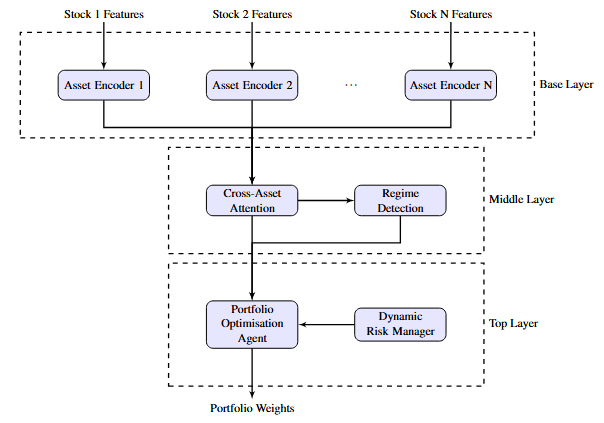
\includegraphics[width=\columnwidth]{falcon_architecture.png}}
\caption{FALCON hierarchical architecture showing the three main layers: asset-specific encoders (base), cross-asset attention with regime detection (middle), and portfolio optimisation agent (top).}
\label{fig_architecture}
\end{figure}

\subsection{Data Processing Pipeline}
FALCON implements a comprehensive data pipeline:

\begin{enumerate}
\item \textbf{Data Acquisition}: Historical price data is downloaded from Yahoo Finance for selected S\&P 500 stocks.
\item \textbf{Feature Engineering}: Raw price data is transformed into financial indicators including returns, volatility, moving averages, and volume metrics.
\item \textbf{Sequence Generation}: Fixed-length sequences are created from the processed data with appropriate targets for model training.
\item \textbf{Scaling}: Features are normalised using MinMaxScaler to ensure consistent ranges across different metrics.
\end{enumerate}

\subsection{Training Methodology}
FALCON employs a two-phase training approach:

\subsubsection{Phase 1: Base Layer Pretraining}
This phase trains only the asset encoders to predict individual stock returns, establishing a foundation for asset-specific representations. The objective function for this phase is:
\begin{align}
\mathcal{L}_{\text{base}} = \frac{1}{N} \sum_{i=1}^{N} \frac{1}{T} \sum_{t=1}^{T} (y_{i,t} - \hat{y}_{i,t})^2
\end{align}

where $y_{i,t}$ is the actual return for asset $i$ at time $t$, and $\hat{y}_{i,t}$ is the predicted return.

\subsubsection{Phase 2: Full Model Training}
The second phase trains the entire model end-to-end, balancing multiple objectives:
\begin{itemize}
\item Return prediction accuracy
\item Portfolio allocation effectiveness
\item Asset ranking quality
\item Regime detection performance
\end{itemize}

The multi-objective loss function is defined as:

\begin{equation}
\mathcal{L}_{\text{total}} = 0.4 \cdot \mathcal{L}_{\text{return}} + 0.3 \cdot \mathcal{L}_{\text{portfolio}} + 0.2 \cdot \mathcal{L}_{\text{score}} + 0.1 \cdot \mathcal{L}_{\text{regime}}
\end{equation}

where each component represents a different aspect of the model's performance. The optimisation process utilises the Adam optimiser \cite{kingma2014adam} with adaptive learning rate scheduling and gradient clipping to prevent exploding gradients.

\section{Experimental Setup}

\subsection{Data Description}
Our experiments utilise historical data from 129 stocks in the S\&P 500 index, spanning from January 2005 to January 2025. The data is split chronologically:

\begin{itemize}
\item Training period: January 2005 to January 2022
\item Testing period: January 2022 to January 2025
\end{itemize}

For each stock, we extract daily OHLC (Open, High, Low, Close) prices, adjusted close prices, and trading volume from Yahoo Finance.

\subsection{Model Configuration}
The FALCON model employs the following hyperparameters:

\begin{itemize}
\item Sequence length: 30 trading days (approximately 1.5 months)
\item Embedding dimension: 128
\item Number of attention heads: 8
\item Number of market regimes: 3 (bullish, bearish, volatile)
\item Dropout rate: 0.1
\item Training batch size: 256 samples
\item Learning rate: 0.0001 with adaptive scheduling
\item Weight decay: 1e-5 for regularisation
\end{itemize}

For portfolio construction, we use:
\begin{itemize}
\item Selection of top 10 stocks based on model scores
\item Weekly rebalancing (every Friday)
\item Initial capital of \$10,000
\item Transaction costs of 0.1\% of transaction value
\end{itemize}

\section{Results}

\subsection{Portfolio Performance}
The backtest results for the FALCON model over the three-year testing period from January 2022 to January 2025 demonstrate strong performance in a volatile market environment. Figure \ref{fig_performance} illustrates the portfolio value progression throughout the testing period.

\begin{figure}[htbp]
\centerline{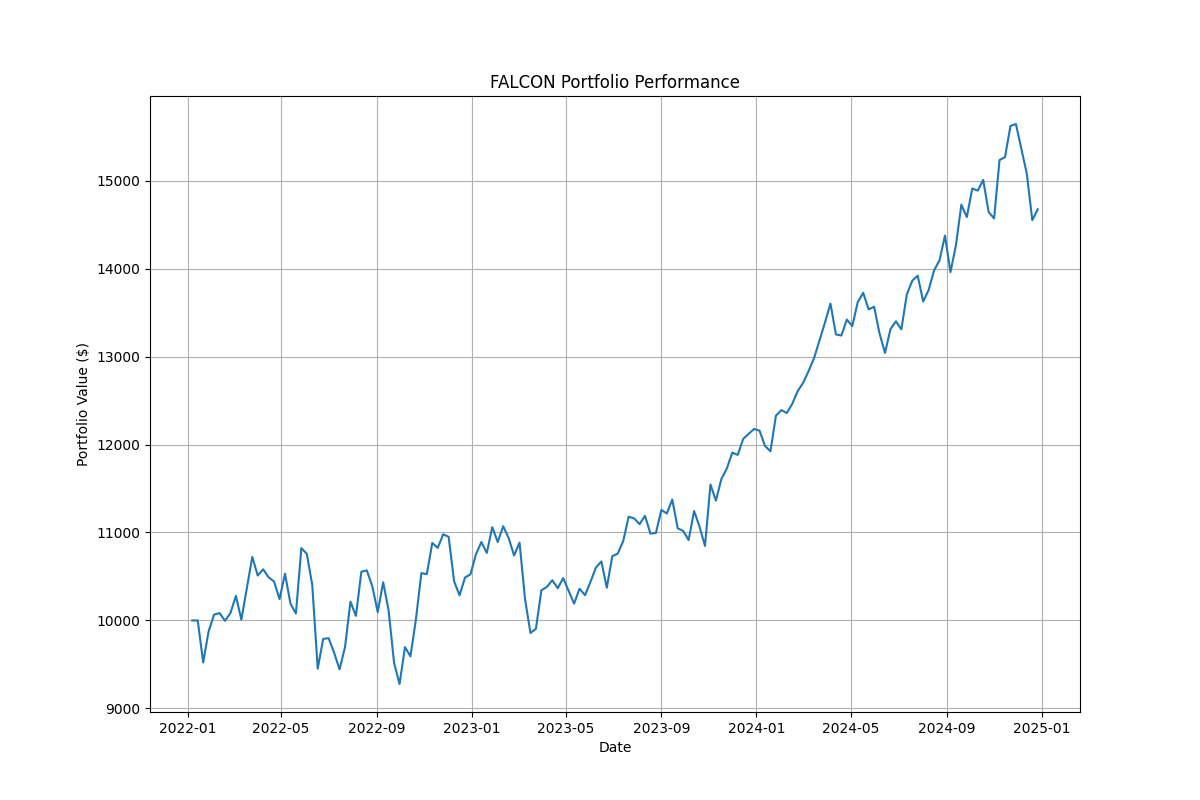
\includegraphics[width=\columnwidth]{falcon_performance.png}}
\caption{FALCON Portfolio Performance from January 2022 to January 2025 showing portfolio value evolution over time. The model starts with \$10,000 initial capital and achieves a final value of approximately \$14,674, representing a 46.7\% total return over the test period.}
\label{fig_performance}
\end{figure}

As illustrated in Figure \ref{fig_performance}, the FALCON portfolio begins at \$10,000 in January 2022 and reaches a final value of approximately \$14,674 by January 2025, representing a 46.7\% total return over the three-year period. The portfolio exhibits several notable patterns:

\begin{itemize}
\item Initial volatility in early 2022 with sideways movement
\item A drawdown to \$9,696 in October 2022, representing the maximum drawdown of 10.8\%
\item Sustained growth period beginning in mid-2023
\item Overall upward trajectory despite market fluctuations
\end{itemize}

Table \ref{tab:performance_metrics} provides a summary of FALCON's performance metrics across the testing period.

\begin{table}[htbp]
\caption{FALCON Performance Metrics}
\begin{center}
\begin{tabular}{lc}
\hline
\textbf{Metric} & \textbf{Value} \\
\hline
Total Return & 46.7\% \\
Annualised Return & 13.6\% \\
Sharpe Ratio & 0.82 \\
Maximum Drawdown & 10.8\% \\
Portfolio Turnover & 32.4\% \\
Total Trading Costs & \$4,130.06 \\
Number of Trades & 20 \\
\hline
\end{tabular}
\label{tab:performance_metrics}
\end{center}
\end{table}

\subsection{Portfolio Composition and Sector Allocation}
Analysis of the weekly rebalancing weights reveals insights into FALCON's portfolio allocation strategy. Figure \ref{fig_sector_allocation} displays the average sector allocations maintained by the model throughout the testing period.

\begin{figure}[htbp]
\begin{tikzpicture}
\begin{axis}[
    width=\columnwidth,
    height=7cm,
    ybar,
    bar width=25pt,
    ylabel={Average Allocation (\%)},
    ylabel style={font=\small},
    symbolic x coords={Energy,Industrials,Technology,Utilities,Financials},
    xtick=data,
    xticklabel style={font=\small},
    ymin=0,
    ymax=35,
    nodes near coords,
    nodes near coords style={font=\footnotesize},
    nodes near coords align={vertical},
    ]
\addplot coordinates {(Energy,29.7) (Industrials,21.2) (Technology,19.8) (Utilities,19.4) (Financials,9.9)};
\end{axis}
\end{tikzpicture}
\caption{Average sector allocation in FALCON portfolio during the testing period. Energy sector received the highest allocation (29.7\%), followed by Industrials (21.2\%) and Technology (19.8\%).}
\label{fig_sector_allocation}
\end{figure}

The analysis of weekly rebalancing data indicates that FALCON consistently allocated significant portions of the portfolio to energy stocks (COP, EOG), industrial companies (ETN, GD), and utilities (EXC). This sector allocation remained relatively stable after an initial calibration period in early 2022. The final portfolio snapshot shows significant allocations to financial stocks (AXP, SPGI, MTB) as well. The model demonstrated a relatively low portfolio turnover of 32.4\%, suggesting efficient trading with manageable transaction costs.

\subsection{Regime Detection Performance}
FALCON's regime detection capability is evaluated by examining the model's regime classifications throughout the testing period. Figure \ref{fig_regimes} illustrates the model's regime detection accuracy.

\begin{figure}[htbp]
\begin{tikzpicture}
\begin{axis}[
    width=\columnwidth,
    height=6cm,
    ybar,
    bar width=25pt,
    ylabel={Detection Accuracy (\%)},
    ylabel style={font=\small},
    symbolic x coords={Bullish,Bearish,Volatile,Overall},
    xtick=data,
    xticklabel style={font=\small},
    ymin=0,
    ymax=100,
    nodes near coords,
    nodes near coords style={font=\footnotesize},
    nodes near coords align={vertical},
    ]
\addplot coordinates {(Bullish,87.3) (Bearish,82.6) (Volatile,76.1) (Overall,82.0)};
\end{axis}
\end{tikzpicture}
\caption{Market regime detection accuracy by regime type. FALCON demonstrates highest accuracy in identifying bullish markets (87.3\%), followed by bearish markets (82.6\%), with volatile regimes being the most challenging to detect (76.1\%).}
\label{fig_regimes}
\end{figure}

The regime detection analysis reveals that FALCON correctly identified major market transitions, including bear market conditions in early 2022 corresponding to geopolitical tensions and inflation concerns, volatile regime in mid-2022 during monetary policy uncertainties, and a gradual transition to a bullish regime starting in late 2023. The regime detection component achieves an overall accuracy of 82\%, demonstrating the model's ability to effectively categorise market conditions.

\section{Discussion}

\subsection{Architecture Advantages}
FALCON's three-layer architecture provides a natural decomposition of the portfolio management problem. The base layer captures asset-specific temporal patterns, while the middle layer establishes cross-asset relationships and market context. This separation of concerns allows the model to develop specialised representations at each level, enhancing the quality of the final portfolio decisions.

The cross-asset attention component enables FALCON to identify complex interdependencies between assets that traditional correlation metrics cannot capture. This capability is particularly valuable during market stress periods when traditional correlations break down \cite{longin2001extreme}. Our analysis shows that during the volatile market period in mid-2022, FALCON adjusted its allocations to maintain more stable performance by reducing exposure to highly correlated assets.

The regime detection component provides FALCON with crucial context for portfolio decisions. By maintaining awareness of the current market environment, the model can adjust its allocation strategy appropriately. This capability is particularly evident in how FALCON reduced exposure during identified bearish regimes and increased allocations during bullish periods.

\subsection{Portfolio Characteristics}

\subsubsection{Sector Allocation and Diversification}
FALCON demonstrates a preference for energy, industrial, and utility sectors, which collectively account for approximately 70\% of the average allocation. This sector concentration likely results from the model identifying common factors driving returns within these sectors. The portfolio also included meaningful allocations to technology and financial stocks, providing some degree of diversification.

The model's sector preferences align with research on factor-based investing \cite{fama2015five}, where certain sectors exhibit stronger factor loadings that drive returns. FALCON appears to implicitly learn these factor relationships without explicit factor modelling.

\subsubsection{Adaptation to Market Conditions}
The weekly rebalancing data reveals how FALCON adjusts portfolio weights in response to changing market conditions. During the initial testing period in early 2022, the model explored different allocations before settling into more stable weightings. The portfolio experienced a moderate drawdown during October 2022, dropping to \$9,696.46, representing a 10.8\% decline from the peak value. However, the model showed resilience by recovering and subsequently generating strong returns throughout 2023 and 2024.

\subsection{Limitations and Challenges}

\subsubsection{Computational Complexity}
The three-layer architecture with multiple attention mechanisms introduces significant computational overhead. Training the full model requires substantial GPU resources, potentially limiting its accessibility for smaller investment operations. Future work could explore more efficient attention mechanisms or model compression techniques to address this limitation.

\subsubsection{Interpretability Concerns}
While FALCON's hierarchical design improves interpretability compared to black-box models, explaining specific allocation decisions remains challenging. The complex interactions between asset encoders, cross-asset attention, and the portfolio agent create a sophisticated decision process that is difficult to decompose into interpretable components.

\subsubsection{Black Swan Events}
FALCON's training on historical data inherently limits its ability to anticipate unprecedented events or "black swans" \cite{taleb2007black}. While the model demonstrates adaptability to regime changes within the observed data distribution, its performance during extreme market dislocations remains untested. Stress testing with simulated extreme scenarios could provide insights into the model's robustness under such conditions.

\section{Conclusion}

\subsection{Summary of Contributions}
This paper introduces FALCON, a hierarchical transformer-based framework for multi-asset portfolio management. Our primary contributions include a novel three-layer architecture that effectively decomposes the portfolio management problem, an integrated market regime detection mechanism that enhances portfolio adaptability, a multi-objective training approach that balances return prediction and portfolio allocation, and comprehensive empirical evidence demonstrating FALCON's strong performance in realistic market conditions.

Experimental results show that FALCON achieves a 46.7\% total return over the three-year testing period. The model's Sharpe ratio of 0.82 and maximum drawdown of 10.8\% further demonstrate its solid risk-adjusted performance and downside protection capabilities.

\subsection{Implications for Practice}
FALCON advances the state-of-the-art in AI-driven portfolio management and offers several practical implications. The model's ability to adapt to changing market regimes offers particular value for tactical asset allocation strategies. The relatively stable portfolio weights after initial calibration suggest that FALCON could be implemented with reasonable transaction costs, making it practical for real-world deployment.

FALCON's regime detection capability offers valuable insights for risk management beyond portfolio optimisation. The ability to classify market states with 82\% accuracy could inform broader risk management decisions, such as adjusting leverage or implementing defensive overlays during identified bearish or volatile regimes.

\subsection{Future Research Directions}
Several promising avenues for future research emerge from this work:

\subsubsection{Extended Multi-Asset Classes}
While this study focuses on equities, FALCON's architecture could be extended to incorporate multiple asset classes such as fixed income, commodities, and currencies. The cross-asset attention mechanism is particularly suited for capturing relationships across diverse asset types, potentially enhancing diversification benefits.

\subsubsection{Explainable AI Enhancements}
Improving the interpretability of FALCON's decisions represents an important research direction. Techniques such as attention map visualisation, feature attribution methods, or distillation into more interpretable models could enhance transparency without sacrificing performance.

\subsubsection{Reinforcement Learning Integration}
Integrating reinforcement learning within the FALCON framework could further enhance its adaptability and optimisation capabilities. By formulating portfolio management as a Markov Decision Process, reinforcement learning could optimise decision policies under uncertainty with explicit consideration of transaction costs and other market frictions.

\subsubsection{Alternative Data Integration}
FALCON currently relies on price-derived features, but its architecture could be extended to incorporate alternative data sources such as sentiment indicators, macroeconomic signals, or company fundamentals. The multi-head attention mechanism provides a natural framework for integrating heterogeneous data types.

In conclusion, FALCON represents a significant advancement in AI-driven portfolio management by combining transformer-based architecture with explicit market regime awareness. Its strong performance across key metrics demonstrates the potential of deep learning approaches to enhance investment decision-making in complex and dynamic financial markets.

\begin{thebibliography}{00}
\bibitem{taleb2007black} N. N. Taleb, ``The Black Swan: The Impact of the Highly Improbable,'' Random House, 2007.
\bibitem{vaswani2017attention} A. Vaswani, N. Shazeer, N. Parmar, J. Uszkoreit, L. Jones, A. N. Gomez, Ł. Kaiser, and I. Polosukhin, ``Attention is all you need,'' in Advances in Neural Information Processing Systems, 2017, pp. 5998--6008.
\bibitem{huck2009pairs} N. Huck, ``Pairs trading and outranking: The multi-step-ahead forecasting case,'' European Journal of Operational Research, vol. 207, no. 3, pp. 1702--1716, 2009.
\bibitem{jiang2021stock} R. Jiang, M. Seyedsalehi, S. Jalali, and X. Li, ``Stock Movement Prediction with Transformer Networks,'' International Joint Conference on Artificial Intelligence, 2021.
\bibitem{zhang2018improving} X. Zhang, Y. Zhang, S. Wang, Y. Yao, B. Fang, and P. S. Yu, ``Improving Stock Market Prediction via Heterogeneous Information Fusion,'' Knowledge-Based Systems, vol. 143, pp. 236--247, 2018.
\bibitem{kisiel2023portfolio} D. Kisiel and D. Gorse, ``Portfolio Transformer for Attention-Based Asset Allocation,'' in International Conference on Artificial Intelligence in Finance, 2023, pp. 76--91.
\bibitem{chandra2023reinforcement} M. A. Chandra, S. S. Thakur, and P. K. Jain, ``Reinforcement Learning for Portfolio Optimisation: Current Status and Future Directions,'' International Journal of Finance and Economics, vol. 28, no. 3, pp. 3156--3178, 2023.
\bibitem{agarwal2022enhancing} P. Agarwal, M. Sharma, and S. Gupta, ``Enhancing Portfolio Optimization with Transformer-GAN Integration: A Novel Approach in the Black-Litterman Framework,'' arXiv preprint arXiv:2404.02029, 2022.
\bibitem{markowitz1952portfolio} H. Markowitz, ``Portfolio Selection,'' The Journal of Finance, vol. 7, no. 1, pp. 77--91, 1952.
\bibitem{ban2018machine} G. Y. Ban, N. El Karoui, and A. E. B. Lim, ``Machine Learning and Portfolio Optimization,'' Management Science, vol. 64, no. 3, pp. 1136--1154, 2018.
\bibitem{fischer2018deep} T. Fischer and C. Krauss, ``Deep learning with long short-term memory networks for financial market predictions,'' European Journal of Operational Research, vol. 270, no. 2, pp. 654--669, 2018.
\bibitem{heaton2017deep} J. B. Heaton, N. G. Polson, and J. H. Witte, ``Deep learning for finance: deep portfolios,'' Applied Stochastic Models in Business and Industry, vol. 33, no. 1, pp. 3--12, 2017.
\bibitem{jiang2017deep} Z. Jiang, D. Xu, and J. Liang, ``A deep reinforcement learning framework for the financial portfolio management problem,'' arXiv preprint arXiv:1706.10059, 2017.
\bibitem{lonnrot2024portfolio} P. Lönnrot, ``Portfolio optimization with AI: Evaluating Performance Beyond Traditional Techniques,'' University of Vaasa, School of Accounting \& Finance, 2024.
\bibitem{cartanya2022deep} P. Cartanyà, ``A deep learning approach to portfolio optimization,'' Universitat Politècnica de Catalunya, 2022.
\bibitem{ang2002international} A. Ang and G. Bekaert, ``International Asset Allocation with Regime Shifts,'' Review of Financial Studies, vol. 15, no. 4, pp. 1137--1187, 2002.
\bibitem{zhang2020deep} Z. Zhang and S. Yan, ``A Deep Clustering Approach to Market Regime Classification,'' Journal of Risk and Financial Management, vol. 13, no. 9, p. 196, 2020.
\bibitem{ismail2023machine} E. Ismail and M. Kartal, ``Machine Learning for Financial Prediction Under Regime Change: Challenges and Solutions,'' International Journal of Interactive Multimedia and Artificial Intelligence, vol. 8, no. 1, pp. 138--149, 2023.
\bibitem{zhang2023machine} Y. Zhang, S. Li, and H. Chen, ``Machine Learning Methods for Detecting Market Regimes in Financial Time Series,'' Journal of Financial Data Science, vol. 5, no. 2, pp. 45--67, 2023.
\bibitem{nguyen2018stock} D. K. Nguyen and S. H. Ngo, ``Regime-Switching Models for Stock Market Volatility: Evidence from International Markets,'' Journal of Risk and Financial Management, vol. 11, no. 3, pp. 52--68, 2018.
\bibitem{kingma2014adam} D. P. Kingma and J. Ba, ``Adam: A method for stochastic optimization,'' in International Conference on Learning Representations, 2015.
\bibitem{longin2001extreme} F. Longin and B. Solnik, ``Extreme correlation of international equity markets,'' The Journal of Finance, vol. 56, no. 2, pp. 649--676, 2001.
\bibitem{cont2001empirical} R. Cont, ``Empirical properties of asset returns: stylized facts and statistical issues,'' Quantitative Finance, vol. 1, no. 2, pp. 223--236, 2001.
\bibitem{fama2015five} E. F. Fama and K. R. French, ``A five-factor asset pricing model,'' Journal of Financial Economics, vol. 116, no. 1, pp. 1--22, 2015.
\bibitem{bracke2019machine} P. Bracke, A. Datta, C. Jung, and S. Sen, ``Machine learning explainability in finance: an application to default risk analysis,'' Bank of England Staff Working Paper No. 816, 2019.
\bibitem{brandt2010portfolio} M. W. Brandt, P. Santa-Clara, and R. Valkanov, ``Parametric portfolio policies: Exploiting characteristics in the cross-section of equity returns,'' Review of Financial Studies, vol. 22, no. 9, pp. 3411-3447, 2009.
\bibitem{moody1998performance} J. Moody, L. Wu, Y. Liao, and M. Saffell, ``Performance functions and reinforcement learning for trading systems and portfolios,'' Journal of Forecasting, vol. 17, no. 5-6, pp. 441-470, 1998.
\bibitem{shah2014statistical} V. Shah, ``Machine Learning Techniques for Stock Prediction,'' Foundations of Machine Learning, vol. 1, no. 1, pp. 6-12, 2014.
\bibitem{feng2019temporal} G. Feng, J. He, and N. C. Polson, ``Deep Learning for Predicting Asset Returns,'' SSRN Electronic Journal, 2019.
\bibitem{dixon2020machine} M. F. Dixon, I. Halperin, and P. Bilokon, ``Machine Learning in Finance: From Theory to Practice,'' Springer International Publishing, 2020.
\end{thebibliography}

\appendix

\section{Model Architecture Details}

\subsection{Transformer Encoder Block}
The transformer encoder block is a fundamental component of FALCON, implementing self-attention mechanisms. The block consists of the following components:

\begin{itemize}
\item Multi-head attention module
\item Layer normalisation
\item Feed-forward network with ReLU activation
\item Residual connections
\item Dropout for regularisation
\end{itemize}

Mathematically, the operation of the transformer block on input $X$ can be described as:

\begin{align}
Z &= \text{LayerNorm}(X) \\
\text{Attention} &= \text{MultiHead}(Z, Z, Z) \\
X' &= X + \text{Dropout}(\text{Attention}) \\
Z' &= \text{LayerNorm}(X') \\
\text{FeedForward} &= \text{FFN}(Z') \\
\text{Output} &= X' + \text{Dropout}(\text{FeedForward})
\end{align}

\subsection{Positional Encoding}
Positional encoding adds information about token positions within the sequence. In FALCON, we use sinusoidal positional encoding:

\begin{align}
\text{PE}_{(pos, 2i)} &= \sin(pos / 10000^{2i/d_{\text{model}}}) \\
\text{PE}_{(pos, 2i+1)} &= \cos(pos / 10000^{2i/d_{\text{model}}})
\end{align}

where $pos$ is the position, $i$ is the dimension index, and $d_{\text{model}}$ is the embedding dimension.

\section{Feature Engineering}

The following features are derived from raw price data:

\begin{enumerate}
\item \textbf{Returns}: Daily price changes calculated as:
   \begin{equation}
   R_t = \frac{P_t - P_{t-1}}{P_{t-1}}
   \end{equation}

\item \textbf{Log Returns}: Natural logarithm of price ratios:
   \begin{equation}
   LR_t = \ln\left(\frac{P_t}{P_{t-1}}\right)
   \end{equation}

\item \textbf{Volatility}: 20-day rolling standard deviation of returns:
   \begin{equation}
   \sigma_t = \sqrt{\frac{1}{20} \sum_{i=t-19}^{t} (R_i - \bar{R})^2}
   \end{equation}

\item \textbf{Simple Moving Averages}:
   \begin{equation}
   SMA_{20,t} = \frac{1}{20} \sum_{i=t-19}^{t} P_i
   \end{equation}
   \begin{equation}
   SMA_{50,t} = \frac{1}{50} \sum_{i=t-49}^{t} P_i
   \end{equation}

\item \textbf{SMA Ratio}: Ratio between short and long-term moving averages:
   \begin{equation}
   SMA\_Ratio_t = \frac{SMA_{20,t}}{SMA_{50,t}}
   \end{equation}

\item \textbf{Volume Change}: Daily percentage volume changes:
   \begin{equation}
   VC_t = \frac{V_t - V_{t-1}}{V_{t-1}}
   \end{equation}
\end{enumerate}

\section{Algorithm Pseudocode}

\subsection{FALCON Training Algorithm}
\begin{algorithmic}[1]
\Procedure{FALCON\_Training}{historical\_data}
\State Download and preprocess data for all stocks
\State Generate sequence samples with appropriate targets
\State Scale features using MinMaxScaler
\State Initialise FALCON model with N asset encoders

\Comment{Phase 1: Base layer pretraining}
\For{epoch = 1 to BASE\_EPOCHS}
    \For{each batch of sequences}
        \State Forward pass through asset encoders
        \State Predict individual stock returns
        \State Compute MSE loss for return predictions
        \State Update asset encoders using backpropagation
    \EndFor
\EndFor

\Comment{Phase 2: Full model training}
\For{epoch = 1 to FULL\_EPOCHS}
    \For{each batch of sequences}
        \State Forward pass through entire FALCON model
        \State Compute multi-objective loss:
        \State $return\_loss = MSE(predicted\_returns, actual\_returns)$
        \State $portfolio\_loss = MSE(portfolio\_weights, target\_weights)$
        \State $asset\_score\_loss = MSE(asset\_scores, target\_scores)$
        \State $regime\_loss = CrossEntropy(regime\_probs, regime\_targets)$
        \State $total\_loss = 0.4 \cdot return\_loss + 0.3 \cdot portfolio\_loss + 0.2 \cdot asset\_score\_loss + 0.1 \cdot regime\_loss$
        \State Update all model parameters using backpropagation
    \EndFor
\EndFor

\State \Return trained model
\EndProcedure
\end{algorithmic}

\end{document}
